\chapter{The Immersed Boundary Method}
Immersed boundary methods are class of techniques in computational fluid dynamics where the governing equations are solved on cartesian grid that does not conform to the shape of the body in the flow. This is opposed to well known body-conformal techniques where the computational mesh accurately represents the shape of the domain. The boundary condition on the immersed surfaces are not applied explicitly, instead an extra forcing function is added to the governing equations or the discrete numerical scheme is updated near the boundary. The immersed boundary technique is in special interest to us since it removes the mesh sensitivity calculation from the analysis. In this chapter we talk about different classes of immersed boundary technique and apply them to a simple problem. The applicability of these methods in the continuum sensitivity analysis is also discussed. At the end of this chapter, we will chose couple of immersed boundary techniques for sensitivity analysis implementation.

% ======================================================================================
\section{Introduction}
When people started to use computational models in the design of systems, it was usually sufficient to include single physics into the design. The simulations were usually based on structural solvers using finite elements analysis (FEA) or computational fluid dynamics (CFD) simulations. The design requirements for different systems has been drastically changed compared to the initial designs where these computational methods have been applied. The requirements such as higher fuel efficiency, improved controllability, higher stiffness to mass ratios and lower radar signature have forced the designers to develop more unconventional configurations. For example, on way to reduce the infra-red signature of the aircraft engine is to remove it from hanging underneath the wing and put it inside of the aircraft. However, by doing this as massive heat source will be added the structure. The thermal expansion due to this excessive heat load needs to be incorporated into the structural analysis of the system. It requires a multidisciplinary analysis combining thermal analysis for heat transfer and structural analysis for thermal expansion and other structural loads \cite{deaton2013stiffening}.

The multidisciplinary analysis is required for many engineering application however the one that is used most is the interaction of fluid and a deformable structure. This is commonly known as a Fluid-Solid Interaction (FSI) problem. Fluid–structure interaction (FSI) problems are dealt with in many different engineering applications, such as fluttering and buffeting of bridges \cite{jain1996coupled}, vibration of wind turbine blades \cite{arrigan2011control}, aeroelastic response of airplanes \cite{farhat2006provably}. FSI problems are also seen in blood flows in arteries and artificial heart valves \cite{sotiropoulos2009review}, flying and swimming \cite{kern2006simulations}. The conventional approach for simulating such problems is the Arbitrary Lagrangian–Eulerian (ALE) method. ALE methods are based on body- conforming grids to track the location of the fluid–structure interface. ALE methods have been applied to many FSI problems however, they are cumbersome if not impossible to apply to FSI problems with large deformations for complicated boundary shapes.

Immersed boundary (IB) methods are considered a separate family of methods used for modelling FSI problems with complicated boundary shapes and large deformations. IB methods, are based on solving the governing equations for fluids on a fixed grid. Although this computational grid can be structured (Cartesian) or unstructured, most methods are based on structured grid. When using structured grid, extremely efficient computational methods can be utilized on to solve the governing equations. The fluid–structure boundaries are represented by a set of independent nodes. The solid boundary effect on the flow is formulated either by introducing fictitious body forces in the governing equations or by locally modifying the structure of the background grid.

IB has several advantages over the ALE methods. Probably the biggest advantage is the simplification of the task of grid generation. Generating body-conformal grid for a complex shape is usually very complicated. The objective is to construct a grid that provides adequate local resolution with the minimum number of total grid points.  This requires a significant input from the user and is an iterative process. For complicated boundaries the unstructured grid approach is better suited however the grid quality is reduced for extremely complicated geometry. In contrast, for a simulation carried using an IB method, grid complexity and quality are not affected by the complexity of the geometry. 

This advantage becomes even more clear for flows with moving boundaries. The ALE approach requires generating a new mesh or deforming the old mesh to match the new boundary shape at each time step. The solution from last time step is also required to be projected to this new computational mesh. Both of the deformation/projection can affect the accuracy, robustness and the computational cost associated the the simulation. On the other hand, the boundary motion in IB method can be handled with rather ease because the computational mesh does not depend on the shape of the boundary. Therefore, although a significant progress in simulating flows using ALE methods has been made in the recent years \cite{lomtev1999discontinuous, farhat2004cfd, cheng2005fluid}, the IB method still remains an attractive alternative for such problems due to its simplicity and cost.

In the following sections of this chapter we first look at the governing equations for the fluid and solid domain. Followed by this different approaches for modelling the follow using IB method are discussed in detail. We apply different IB techniques to a simplified problem to compare the efficiency and simplicity of implimentation. The results are compared with body-conformal solution approach for accuracy comparison. Finally we assess different IB methods with regards to their applicability of the Continuum Sensitivity Analysis (CSA) framework.

% ======================================================================================
\section{Governing Equations}
In the fluid region $\Omega_f$, the governing equations for incompressible flow of a Newtonian fluid are known as Navier-Stokes (NS) equations. In the compact indicial notation, the NS equations are written as

\begin{subequations}\label{eq:C3_GE}
\begin{equation}\label{eq:C3_continuity}
	\frac{\partial u_i}{\partial x_i} = 0
\end{equation}
\begin{equation}\label{eq:C3_momentum}
	\frac{\partial u_i}{\partial t} + \frac{\partial u_i u_j}{\partial x_j} = 
	-\frac{1}{\rho_f	} \frac{\partial p}{\partial x_i} + 
	\nu \frac{\partial}{\partial x_j} \left( \frac{\partial u_i}{\partial x_j} \right) + 
	f_i
\end{equation}
\end{subequations}

where the repeated indices imply summation and $i,j=1,2,3$. $x_i$ are the spatial coordinates, $u_i$ are the velocity components of the fluid in $i$ direction, $\rho_f$ is the fluids density, $p$ is the pressure, $\nu$ is the kinematic viscosity, and $f_i$ are body forces. These forces are used in the IB technique to represent the effect of immersed boundaries on the fluid. In general purpose CFD solvers, due to the use of unstructured grid to represent the shape, it is usually required to use mappings (Jacobian) to convert the physical coordinate the a computational coordinate. This will become problematic when we have skewed elements with cause the mapping become singular. This step is removed in the IB approach since the governing equations \eqref{eq:C3_GE} are discretized on a Cartesian  grid.

The solid domain is modelled using linear elastic theory in this work. The governing equations are written as

\begin{subequations}\label{eq:C3_linearEalsticityEquations}
\begin{equation}
	\sigma_{ji,j} + F_i = \rho_s \partial_{tt} u_i
\end{equation}
\begin{equation}
	\epsilon_{ij} = \frac{1}{2} \left( u_{j,i} + u_{i,j} \right)
\end{equation}
\begin{equation}
	\sigma_{ij} = C_{ijkl} \epsilon_{kl}
\end{equation}
\end{subequations}

where $\sigma$ is the Cauchy stress tensor, $\epsilon$ is the strain tensor, $u$ is the displacement vector, $C$ is stiffness tensor, $F$ is the body force, and $\rho_s$ is the mass density of solid. These governing equations are solved to track the motion of of the solid boundary. 

To solve the coupled system of equations of \eqref{eq:C3_GE} and \eqref{eq:C3_linearEalsticityEquations} we need to have boundary conditions. The boundary conditions of \eqref{eq:C3_GE} are defined as pressure or velocity magnitudes on the outer boundaries of the domain. After solving Equation \eqref{eq:C3_GE}, the loads on the structure can be calculated by integrating the pressure from the fluid solid over the solid boundaries. This will be the boundary load used for solving Equation \eqref{eq:C3_linearEalsticityEquations}. When the governing equation for the solid region is solved, the displacement of the solid domain is known. This is fed into the CFD solver to update the solid boundary location for fluid domain. This will change the solution of fluid's solver resulting in different pressure distribution. This process is repeated until a convergence is satisfied. The convergence can be defined as change in the structure deflection for two subsequent steps for a static problem.

% ======================================================================================
\section{Benchmark Case}
We define a 1D benchmark problem to investigate different IB formulations in detail. In one dimensional space the equations of incompressible flow are not very interesting and it is not simple to write a one-dimensional analogue of the IB to capture all of its features. However, for a simple one dimensional problem we can understand different formulations of IB method and later apply it to higher dimensions. Moreover, for the sake of sensitivity analysis better understanding of the problem can be achieved for a simplified model. The other reason for working with a simplified model is the availability of analytical results that can be used for verifying the results we get from the numerical solvers. As the final note, for this benchmark case we mainly focused on the fluid domain, the structures can be easily added to this formulation.

To derive the one dimensional benchmark case we start with the Navier-Stokes equations. Consider a viscous incompressible fluid in the channel $0 \geq y \leq 1$, $-\infty < x < \infty$ as shown in Figure \ref{fig:C3_benchmarkCase}.

\begin{figure}[h]
	\centering
	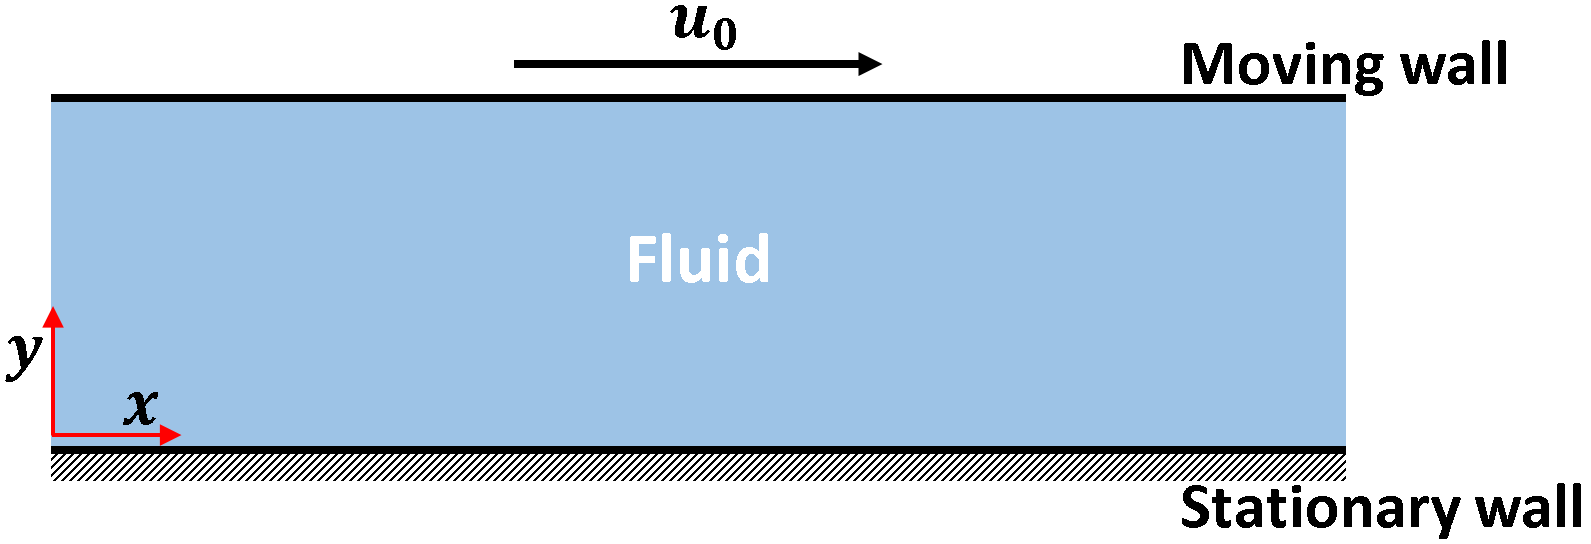
\includegraphics[width=14.00cm]{Chapter_3/figure/C3_infinite_channel.png}
	\caption{1D benchmark case for IB method.}
	\label{fig:C3_benchmarkCase}
\end{figure}

We can also assume that the boundary conditions are periodic in $x$. Next suppose that there is a horizontal plate running through the length of this channel at $y=y_0$ and moving with $u_0$ velocity in horizontal direction. We assume no-slip condition where the fluid and the plate meet. This will force the fluid to accelerate in $x$ direction due to the viscous stress from the moving plate. We expect no motion in $y$ direction and can drop all terms in the NS equations containing $u_j$ velocity. Due to the continuity equation \eqref{eq:C3_continuity}, there is no variation in the $x$ direction so we can drop all the terms that involve with $x$ variation as well. This enables us to simplify the NS equation of \eqref{eq:C3_momentum} into Equation \eqref{eq:C3_benchmarkProblem}. It should be noted that the continuum equation \eqref{eq:C3_continuity} is automatically satisfied.

\begin{subequations}\label{eq:C3_benchmarkProblem}
\begin{equation}
	u_t = \mu u_{yy} \quad \text{in } \Omega_f
\end{equation}
\begin{equation}
\begin{cases}
	u = u_0 \quad \text{at } y = 1 \\
	u = 0 \quad \text{at } y = 0
\end{cases}
\end{equation}
\end{subequations}

Equation \eqref{eq:C3_benchmarkProblem} is transient in nature however, its steady state solution can be calculated by setting the time derivative equal to zero. This equation governs what is commonly known as Couette flow in introductory courses in fluid dynamics. The analytical solution for this equation is shown in Equation \eqref{eq:C3_benchmarkAnalyticalSolution}.

\begin{equation}\label{eq:C3_benchmarkAnalyticalSolution}
	u = u_0 x
\end{equation}

We will use this analytical solution to verify the result of the different IB methods defined in the following sections.

% ======================================================================================
\section{Immersed Boundary Methods}